% Modeled after the following
% A simple Tree
% Author: Stefan Kottwitz
% https://www.packtpub.com/hardware-and-creative/latex-cookbook
\documentclass[border=10pt]{standalone}
\usepackage{tikz}
\begin{document}
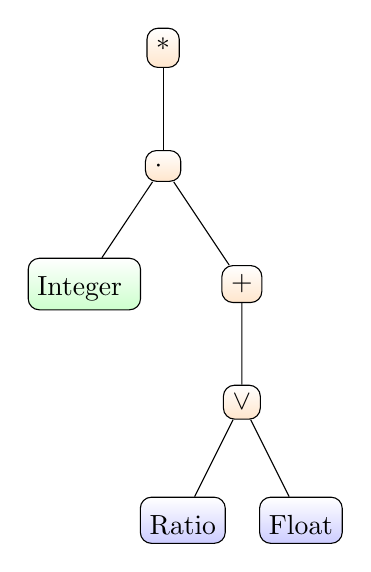
\begin{tikzpicture}[sibling distance=10em,
  every node/.style = {shape=rectangle, rounded corners,
    draw, align=center,
    top color=white, bottom color=orange!20}]]
    \tikzstyle{level 1}=[sibling distance=40mm]
    \tikzstyle{level 2}=[sibling distance=20mm]
    \tikzstyle{level 3}=[sibling distance=15mm]
  \node {*}
  child { node { $\cdot$ } 
    child { node [text height=10pt, bottom color=green!20] { Integer } }
    child { node {$+$} 
      child { node {$\vee$}
        child { node [text height=10pt, bottom color=blue!20] {Ratio} }
        child { node [text height=10pt, bottom color=blue!20] {Float} } } } } ;
\end{tikzpicture}
\end{document}
